\subsection{Story: Site should be mobile responsive}
\subsubsection{Analysis - breakdown of tasks}
\begin{itemize}
	\item Create standard media query sizes
	\item Create media query for quiz questions
	\item Media query for welcome page
\end{itemize}
\subsubsection{Design}
A quiz page should look like the design specified in iteration 4, figures (\ref{fig:iter-4-use-case}).
\subsubsection{Implementation}
For the media query sizes, Bootstrap recommends some default sizes for phones, tablets etc\cite{bootstrap-media-queries}. The Chrome developer tools were used to view the page in mobile view and change the various sizes of buttons and titles in the CSS editor to be more mobile friendly.
\subsubsection{Testing}
This was not really possible to test with Dusk or unit tests, but should be easy to test with users later in the project. Additionally once live the system could be tested using the Google Responsive Test that gives a score for the mobile usability.
\newpage

\subsection{Part two re-design}
Part two involved streaming slides to students with embedded question and was originally planned to be an extension to Microsoft PowerPoint or a similar technology, such as Libre Office. However, after some further research this work was determined to be too large. This meant an alternative solution had to be devised or some extra requirements had to be added to the system. An alternative solution was found rather than abandon the idea of having slides within the quizzes. Slideshow programs usually have the ability to render their slides as PDF, a format which is more heavily supported compared to a propriety format such as .pptx provided by Microsoft. If a PDF is uploaded to the application, PHP could be used to turn these slides into images, which can then be placed on the quiz pages.

This new approach meant some changes to the original stories for the second part, here are the revised stories:
\begin{itemize}
	\item (1) The admin creates slides in their preferred editor and exports them as a PDF
	\item (4) The admin can upload these slides to a quiz they have created in the past
	\item (3) The admin can reorder the questions within the quiz to move them around the slides
	\item (2) When this quiz is run, it should render the slides as well as questions in the order specified
\end{itemize}

There are some disadvantages to this however. The main issues are that slide animations are not rendered as separate slides on the PDF. There are extensions for Microsoft PowerPoint that let the slides be rendered with animations occupying separate slides so as to provide a "fake" animation. Another problem is that the slides would have to be uploaded before a lecture as it can take a few minutes to render PDF slides as images. This could be argued to be an advantage however, if lecturers upload their slides before a lecture they only need to log in to the application when they want to run them. They need not carry the slides on a memory stick or save them to their University storage.
\newpage

\subsection{Story: The admin can upload these slides to a quiz they have created in the past}
\subsubsection{Analysis - breakdown of tasks}
\begin{itemize}
	\item Upload pdf slides
	\item Convert these slides to images
	\item Save references to these slides in the database
	\item Show the slides on the Quiz.show page
\end{itemize}
\subsubsection{Design}
See \ref{fig:iter-7-use-case}

\begin{figure}[H]
	\caption{Use case for quiz creation featuring moving questions and the add slides function. See Iteration 2 for more detailed use case diagram of the rest of the backend.}
	\centerline{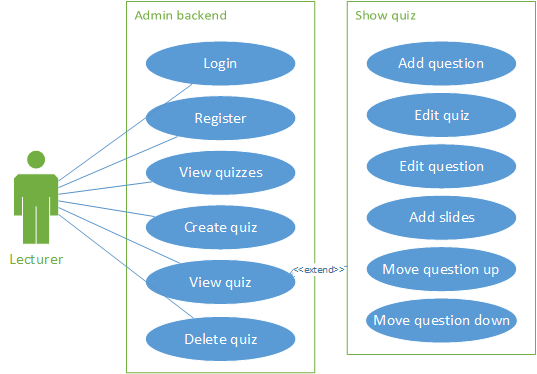
\includegraphics{Chapter2/Iter-7/iter-7-use-case}}
	\label{fig:iter-7-use-case}
\end{figure}

\subsubsection{Implementation}
To upload the slides, it was done with a standard HTML file input but the backend used techniques native to Laravel\cite{laravel-saving-files}. These images were then saved in the /storage/app/public/slides folder. Within this, they were organised into folders named after the session id and then quiz id within those.

These slides were then converted using a library that uses Imagick\cite{spatie-pdf-converter}. A problem is that the details of these images are not kept track of, so after saving the images, references were also saved to a new table in the database. This is so that the images can be referenced quickly later on when displaying a slide. The new table was called slides which stores the file name, quiz it was associated with and a position. 

The last task involved showing the slides and questions on the Quiz.show page. Seeing as one of the other new stories involved reordering questions, merely rendering the slides after the questions would not do. Both the slides and questions needed to be rendered in order of their positions. Unfortunately, there exists no simple SQL query that can select two sets of results and then order them by a common column. The easier solution was to create a PHP function to create an array of all the items in the order required, see appendix \ref{appendix:code} for the function.
\subsubsection{Testing}
There does not appear to be the capacity to upload files in Dusk tests, making this impossible to test unfortunately.
\newpage

\subsection{Story: The admin can reorder the questions within the quiz to move them around the slides}
\subsubsection{Analysis - breakdown of tasks}
\begin{itemize}
	\item Add buttons to reorder questions
	\item This button increases or decreases position of question
	\item The button swaps the positions of two questions or a slide and question if required
	\item Add some limits to positioning such as not going below 1
\end{itemize}
\subsubsection{Design}
As a minor change to the system, no major design choices were made. Simple Bootstrap icons can be used for the position changing arrows, which was the only front end change.
For the newest use case see figure \ref{fig:iter-7-use-case}.
\subsubsection{Implementation}
The main functionality to add was the changing of positions. This involved adding a new route and buttons that triggered the actions associated with this new route. It was decided that the Route would be a POST request rather than GET as the button is submitting some data, the direction and id of the question. The action that was called updates the position in the database after doing some checks of the position it wants to move to. The problem here is that there might be a slide or question occupying that position already, therefore it needs to be checked and swapped if true.
\subsubsection{Testing}
Again as there are no slides it is not fully testable. However, it was possible to test that the questions positions changed in the database when the buttons were clicked without any slides on the page.
\newpage

\subsection{Story: When the quiz is run, it should render the slides as well as the questions in the order specified}
\subsubsection{Analysis - breakdown of tasks}
\begin{itemize}
	\item Find the position in the database and decide whether its a slide or question
	\item If it is a question, render it like before
	\item If a slide, render a simple img tag and populate with the image name from the WebSockets
	\item Resize image to fit the page, including for mobile responsive
	\item Render question by default for users joining late
\end{itemize}
\subsubsection{Design}
This should work in much the same way as the questions, in that it will send an Ajax request to a page with the image name and then copy the content of the Ajax page into the live page. The content page to Ajax should be a simple container with an img tag. The other tasks are extensions to previously created functions.
\subsubsection{Implementation}
The first task was to determine what is at the position. This involved changing the current function to include a check for if the question at the requested position was null. If it was then it should find a slide at the specified position instead of a question. As well as the data about the slide or question, it would return a type so that when it was called the system knew what type of content was expected. The data was then sent to the WebSockets and another case was added to the JavaScript receiving end for triggering an Ajax call to a slide page. This page renders a simple img tag with the slide specified which was then added to the current page, similar to the way questions are rendered.

A problem with rendering the images was that files are stored within the /storage folder which was not publicly accessible. Usually only files within the /public folder are. However, there is an artisan command, \textit{php artisan storage:link}, that creates a symbolic link from the public folder to the storage/app/public folder. This meant that the images could be accessed via /storage/ when specifying the image path.
\subsubsection{Testing}
Given that slides cannot be uploaded, testing for them is not really practical and would involve leaving some test data on the system permanently.
\newpage